\begin{figure}[htbp]

\begin{center}
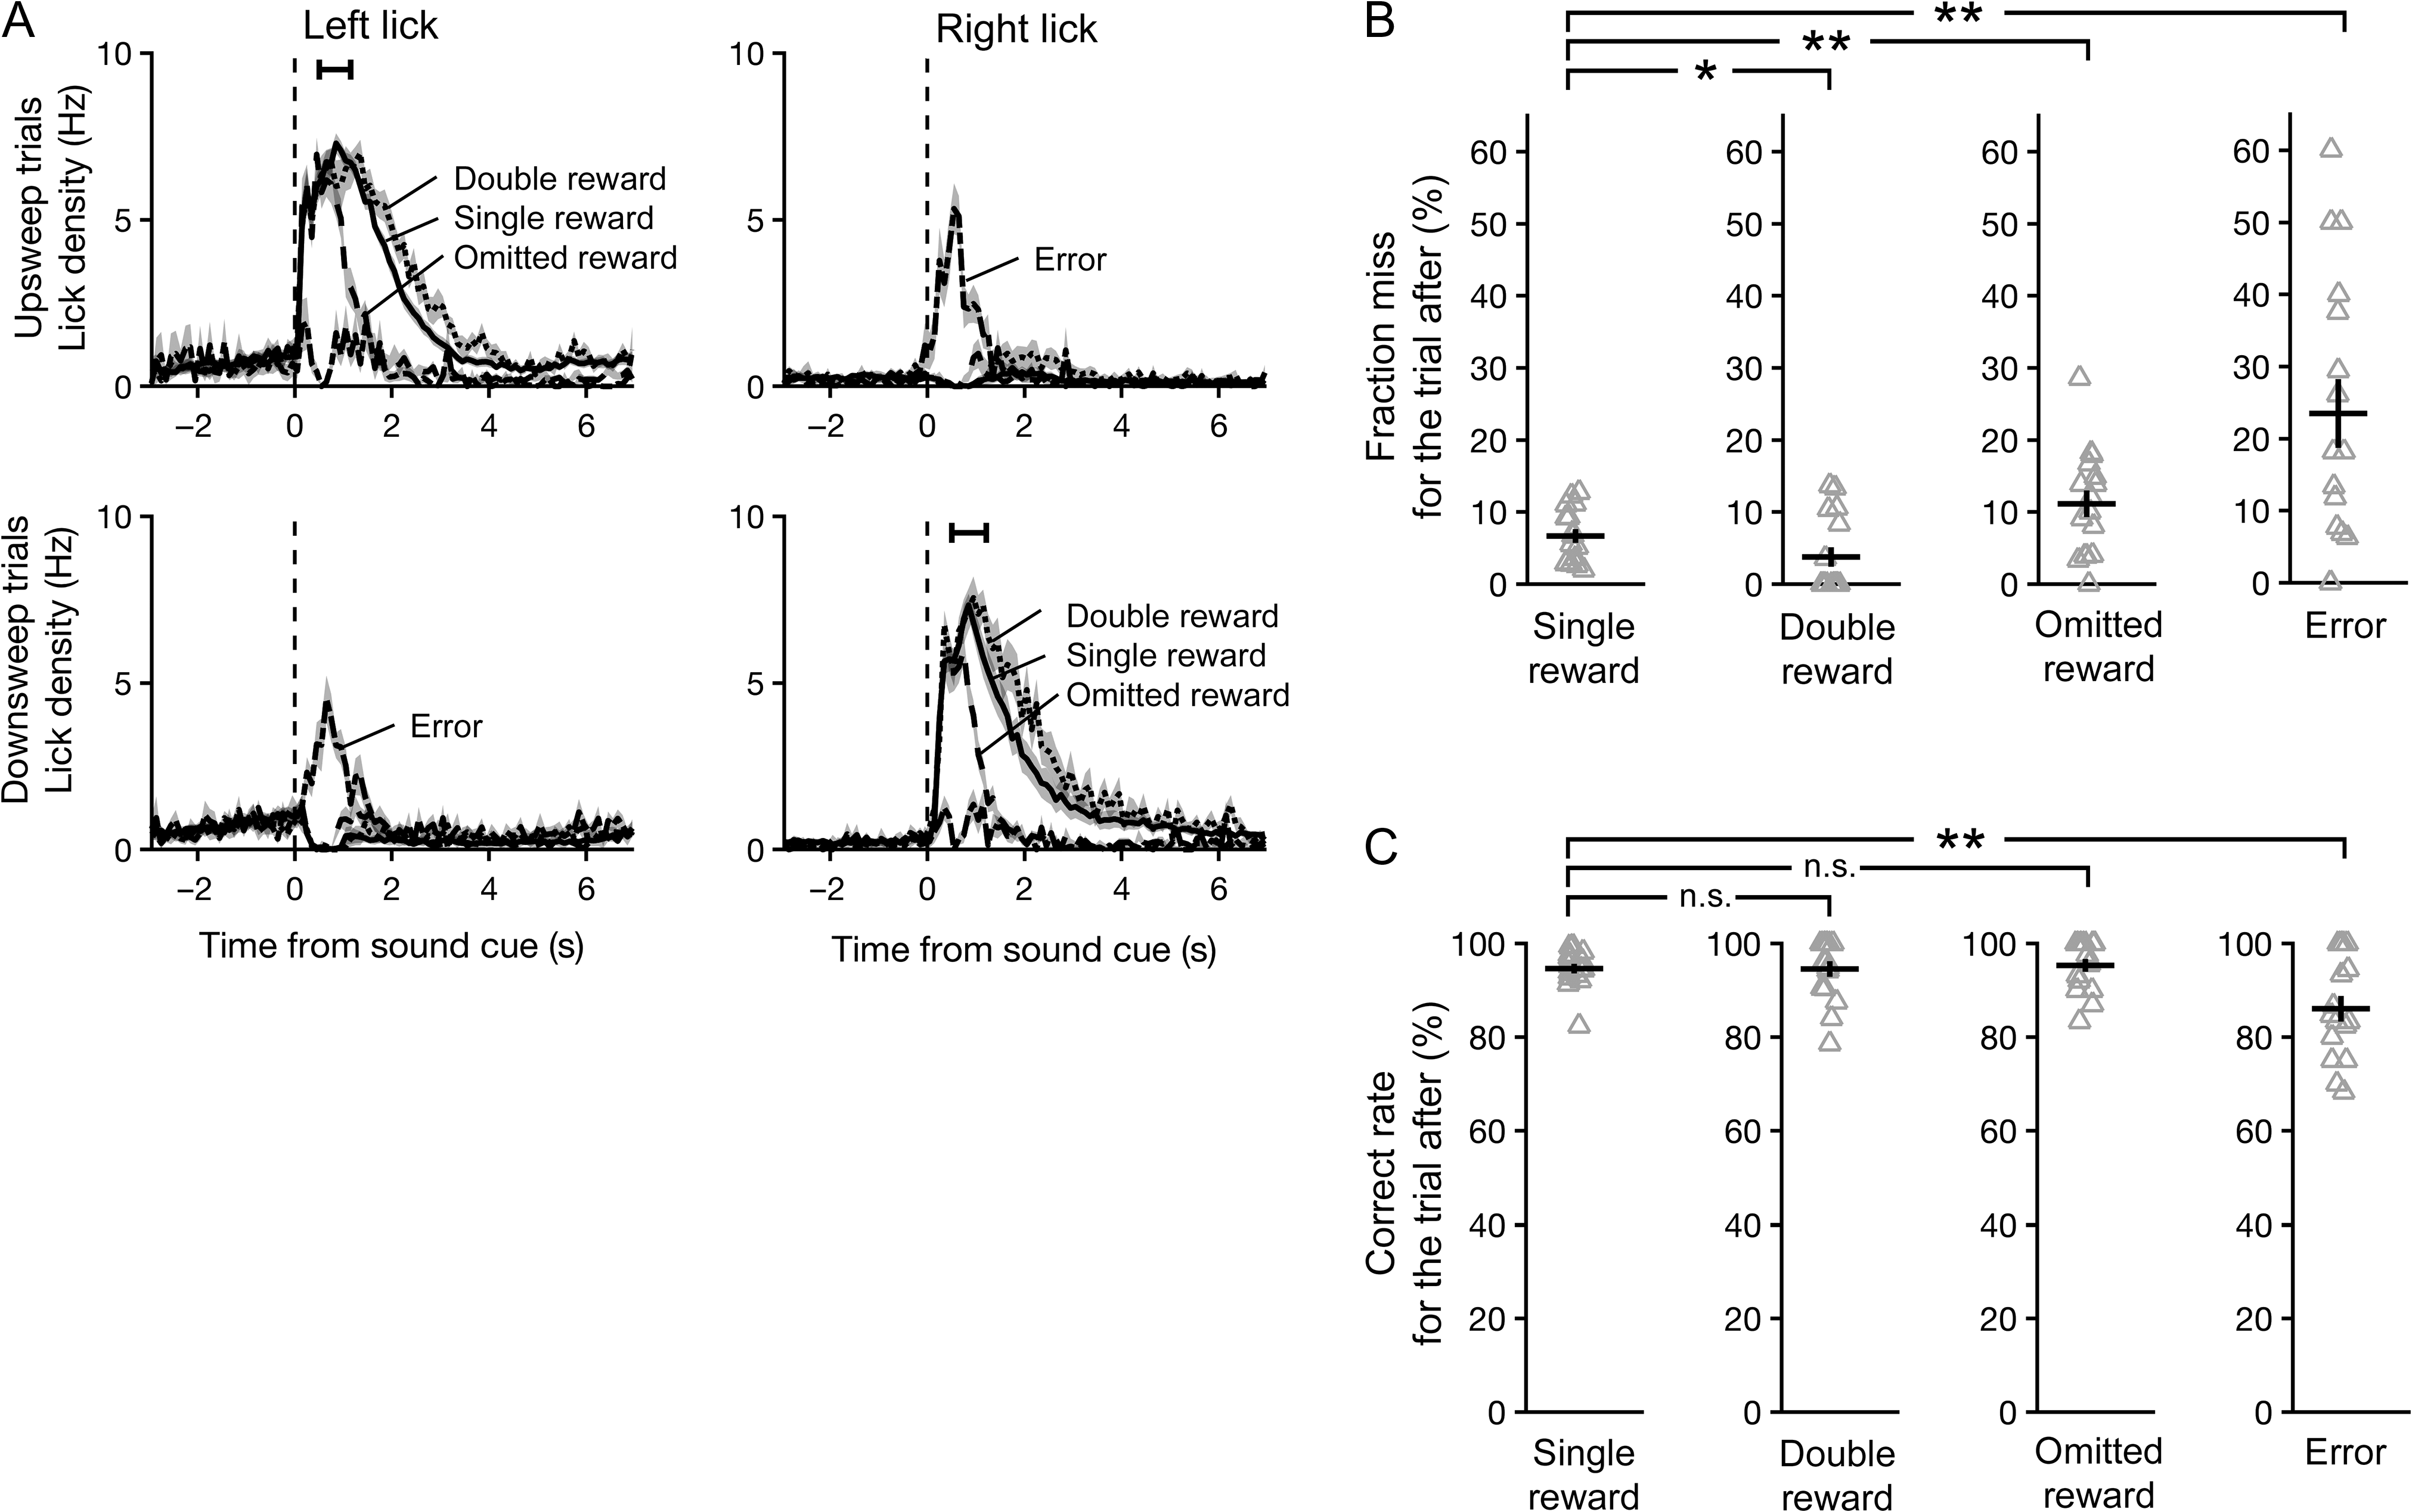
\includegraphics[width=\textwidth]{Figures/CC_fig2.png} 
\end{center}

\caption[Outcome-dependent behavioral adjustments]
{Subjects adjusted their behavior based on trial outcome. (A) Mean lick density across sessions as a function of time for the left and right spouts, averaged separately from trials in which the sound cue was an upsweep (top row) or downsweep (bottom row), and outcome was single reward (solid), double reward (dotted) or omitted reward (dashed). Black error bar, 95\% confidence interval for time of outcome. (B) Fraction of trials missed immediately following each outcome. Gray triangles, individual sessions. Black crosshairs, $mean \pm SEM$. Wilcoxon signed-rank test: *$P < 0.05$, **$P < 0.005$, n.s., not significant. (C) Fraction of trials with a correct response immediately following each outcome.}

\label{fig:CC_fig2}
\end{figure}